% Use only LaTeX2e, calling the article.cls class and 12-point type.

\documentclass[12pt]{article}

% Users of the {thebibliography} environment or BibTeX should use the
% scicite.sty package, downloadable from *Science* at
% www.sciencemag.org/about/authors/prep/TeX_help/ .
% This package should properly format in-text
% reference calls and reference-list numbers.

\usepackage[sort]{scicite}
\usepackage{times}
\usepackage{graphicx}
\usepackage{lineno}
\usepackage{color}
\usepackage{multirow}

% The following parameters seem to provide a reasonable page setup.

\topmargin 0.0cm
\oddsidemargin 0.2cm
\textwidth 16.5cm 
\textheight 21cm
\footskip 1.0cm


%The next command sets up an environment for the abstract to your paper.

\newenvironment{sciabstract}{%
\begin{quote} \bf}
{\end{quote}}


% If your reference list includes text notes as well as references,
% include the following line; otherwise, comment it out.

%\renewcommand\refname{References and Notes}

% The following lines set up an environment for the last note in the
% reference list, which commonly includes acknowledgments of funding,
% help, etc.  It's intended for users of BibTeX or the {thebibliography}
% environment.  Users who are hand-coding their references at the end
% using a list environment such as {enumerate} can simply add another
% item at the end, and it will be numbered automatically.

\newcounter{lastnote}
\newenvironment{scilastnote}{%
\setcounter{lastnote}{\value{enumiv}}%
\addtocounter{lastnote}{+1}%
\begin{list}%
{\arabic{lastnote}.}
{\setlength{\leftmargin}{.3in}}
{\setlength{\labelsep}{.5em}}}
{\end{list}}


% Include your paper's title here

\title{The Spatial and Temporal Domains of Modern Ecology }%\\
%OR Ecology's Spatio-temporal Domains\\
%OR Space, Time, and Ecology \\
%OR Ecology: still a small-scale, field-based discipline} 
 
\author
{Lyndon Estes$^{\ast1, 2, 3}$, Paul R. Elsen$^{2, 4}$, Tim Treuer$^{5}$, Labeeb Ahmed$^{6}$, \\
Kelly Caylor$^{3, 7}$, Jason Chang$^{6}$, Jonathan J. Choi$^{5}$, and Erle Ellis$^{6}$ \\
\\
\normalsize{$^{1}$Graduate School of Geography, Clark University, Worcester MA 01610, USA}\\
\normalsize{$^{2}$Woodrow Wilson School, Princeton University, Princeton, NJ 08544, USA}\\
\normalsize{$^{3}$Civil and Environmental Engineering, Princeton University, Princeton, NJ 08544, USA}\\
\normalsize{$^{4}$Department of Environmental Science, Policy, and Management,}\\
\normalsize{University of California Berkeley, Berkeley, CA 94720, USA}\\
\normalsize{$^{5}$Ecology and Evolutionary Biology, Princeton University, Princeton, NJ 08544, USA}\\
\normalsize{$^{6}$Geography and Environmental Systems, University of Maryland Baltimore County,}\\ 
\normalsize{Baltimore, MD 21250, USA}\\
\normalsize{$^{7}$Earth Research Institute, University of California Santa Barbara, Santa Barbara, CA 93106, USA}\\
\\
\normalsize{$^\ast$To whom correspondence should be addressed; E-mail:  LEstes@clarku.edu.}}
% Include the date command, but leave its argument blank.

\date{}



%%%%%%%%%%%%%%%%% END OF PREAMBLE %%%%%%%%%%%%%%%%



\begin{document} 

% Double-space the manuscript.

\baselineskip24pt

% Make the title.

\maketitle 

\section*{Abstract}
\textbf{To properly understand ecological phenomena, it is necessary to observe them across a range of spatial and temporal scales. Ecologists first raised this point in the 1980s, and since then the ability to collect multi-scale observations has grown rapidly. To assess modern ecology's progress in addressing scale, we analyzed the resolution, extent, interval, and duration of observations in 348 observational studies published between 2004-2014. We found that the scale domains of observations are fairly narrow, and are collected primarily with conventional field techniques. In the spatial domain, most observations have resolutions of $\leq$1 m2 and extents of $\leq$10,000 ha. In the temporal domain, most observations were either unreplicated or of low frequency ($\geq$1 month interval), and were made over relatively short durations ($\leq$1 year). Compared to prior meta-analyses from the 1980s and early 2000s, observational durations and resolutions remain largely unchanged, but intervals have become finer and extents larger. Despite such gains, a large gulf exists between the scales at which phenomena are actually observed, and the scales those observations ostensibly represent, revealing portions of space and time not truly captured by replicates and raising concerns about observational comprehensiveness. Adding to these concerns, scales were not clearly reported in most studies, suggesting that it is a minor consideration. Journals can help mitigate this problem by implementing scale reporting standards, which can spur ecologists to more rapidly adopt new observational technologies, and thereby close key gaps in current observational domains.} 


\linenumbers
\vspace{10pt}
The scales at which ecosystems are observed plays a critical role in shaping our understanding of their structure and function \cite{levin_problem_1992,chave_problem_2013,wiens_spatial_1989}.  Ecological patterns emerge from temporal and spatial domains that may be coarser or finer than the processes that shape them, which means that investigation across multiple scales is essential for understanding ecological phenomena \cite{levin_problem_1992}. This awareness has grown rapidly since the 1980s, accelerated by the need to understand how changes in the global climate, ocean, and land systems are affecting everything from individual populations \cite{tingley_push_2012} to entire biomes \cite{xiao_photosynthetic_2004}, while technological advances in areas such as remote sensing and genetics are making it ever-easier to quantify ecological features across a broad and increasing range of scales \cite{schneider_rise_2001, chave_problem_2013}.  

Given the growing awareness of scale, expanding data gathering capabilities, and the fact that the most comprehensive (and arguably best-known) meta-analyses of ecological research scales were published nearly 30 years ago \cite{tilman_ecological_1989,kareiva_spatial_1988}, it is both timely and important to assess the scales of contemporary ecological investigation. To address this need, we quantified the spatial and temporal domains (here domain means the distribution of observations within the spectrum of one or more scale dimensions\footnote{This definition differs slightly from Wiens' \cite{wiens_spatial_1989}, who defined ``domain of scale'' as ``a portion of the scale spectrum within which process-pattern relationships are consistent regardless of scale.''}) of empirical observations (defined here as ecological observations collected under un-controlled or non-manipulated conditions) that were reported within recently (2004-2014) published ecological studies. Empirical observations are critical for developing and testing the models that explain why ecological patterns vary in time and space \cite{levin_problem_1992, tilman_ecological_1989}, therefore the spatio-temporal domains of observations provide an important indicator of the field's progress towards achieving a holistic, predictive understanding of ecosystems \cite{chave_problem_2013,levin_problem_1992}. 

Our analysis focused on two dimensions of spatial scale, resolution (grain) and extent, and two of temporal scale, interval and duration (Table 1, and see SI for full definitions). Resolution is the area of an individual spatial replicate within which a complete measurement (as opposed to a sub-sample) of the feature of interest was made. Extent is the area enclosed by the outer-most spatial replicates, or, if the system or habitat being sampled was distinct from its surrounding matrix (e.g. forest patches in grassland habitats), the summed area of sampled patches. Interval refers to the average time elapsed between individual temporal replicates. Duration measures the time elapsed between the first and last temporal replicates, or, in the case of temporally unreplicated observations, the estimated time spent collecting the observation. We also assessed observational scales within two additional dimensions, \emph{actual} extent (the summed area of spatial replicates) and \emph{actual} duration (the summed observational time of temporal replicates). We evaluated these additional dimensions to gain insight into how much the actual scales of observation (i.e. how much space and time is covered by the measurement) differ from the scales that the observations are explicitly or implicitly intended to represent. This difference may contain important information about how effectively ecological observations characterize ecological phenomena. First, an increasing gap between actual and intended observational scale inherently implies greater interpolation or extrapolation of observed measurements, raising the odds of over-leveraging data. Second (and relatedly), since natural systems are frequently complex, non-linear, and non-random \cite{levin_ecosystems_1998,pringle_spatial_2017,rietkerk_regular_2008}, a larger gap may increase the likelihood of encountering unanticipated data challenges such as censored data (\emph{sensu} \cite{efron_efficiency_1977}), as phenomena may resolve themselves in the space or time between observations. 

\begin{table}[htp]
\caption{The scale dimensions of ecological observations assessed in this meta-analysis.}
\begin{center}
\begin{tabular}{llll}
\hline
\multicolumn{2}{c}{\textbf{Component}} & \textbf{Units} & \textbf{Description} \\\hline\hline
\multirow{3}*{Spatial} & Resolution & m$^2$ & Area of an individual spatial replicate (e.g. plot) \\%\cmidrule(l){2-3}
   & Extent & ha & Area  encompassed by all spatial replicates \\
   & Actual extent & ha & Summed area of all spatial replicates\\\hline
\multirow{3}*{Temporal} & Interval & days & Time elapsed between successive temporal replicates \\
   & Duration & days & Time elapsed between first and last temporal replicates\\
   & Actual duration & days & Summed observational time of all temporal replicates\\
\hline
\end{tabular}
\end{center}
\label{default}
\end{table}%

%We extracted these scale dimensions from 379 observations that were reported in 134 papers that were published between 2004-2014 in the top 30 (based on 2012 impact factor) ecology-themed journals. 
%

Our analysis was based on a review of 348 papers randomly selected from 42,918 published between 2004-2014 in the top 30 (based on 2012 impact factor) ecology-themed journals. We extracted scale data from 378 observations of ``natural'' (i.e. non-experimentally manipulated) ecological features that were reported within 133 of the reviewed papers (plus an additional 62 that these cited as the source of observations). We excluded experiments because they tend to be of limited extent, duration, and resolution due to their higher logistical costs \cite{tilman_ecological_1989, kareiva_spatial_1988}, and would therefore likely bias our findings towards finer scales, while minimizing the impact that new observing methods (e.g. satellite imaging, wireless sensing) may have had in expanding the scales of ecological investigation \cite{turner_remote_2003,pettorelli_satellite_2014,porter_wireless_2005}. 

To account for uncertainty in the estimation of observational dimensions due to 1) unclear methodological description in the reviewed papers, and 2) observer interpretation, we conducted a resampling analysis (n=1000) in which scale values were randomly perturbed within the bounds of estimated inter-observer variation (SI). We constructed histograms for each dimension from the mean of the perturbed ensembles, and estimated 95\% confidence intervals for each histogram bin (Fig. 1). We constructed kernel density estimates from the full resampled ensemble in order to assess observational distributions within different juxtapositions of the four primary (resolution, extent, interval, duration) space-time dimensions (Fig. 2). 

\noindent \textbf{Results}\\
\noindent \textbf{\emph{Observational methods}}\\
To account for potential differences in scales related to methodology, we classified each observation according to the following broad categories, which were field methods (manual \emph{in situ} data collection), automated (\emph{in situ}) sensing, remote sensing/other geographic data, and paleo-reconstruction approaches. Field methods were used for 80\% of observations, automated sensing for 12.4\%, remote sensing for 6.9\%, and paleo-reconstruction for less than 0.8\%. 

\noindent \textbf{\emph{Domains}}\\
In terms of resolution, the majority (67\%) of observations (across all methods) were collected in plots of $<$1 m$^2$ resolution, 24\% were collected within plots of 1 m$^2$ up to 1 ha, and the remaining 9\% in plots of $\geq$1 ha (Fig. 1A). These distributions primarily reflect those of field observations, the dominant observational methodology. Examining the distributions for each observational method (Fig. S1 in SI) shows that automated sensing and paleo-reconstruction had resolutions that were generally finer ($<$0.1 m$^2$) than field observations, while remote observations were generally coarser ($>$100 m$^2$).   

The extent of 19\% of observations was $<$10 ha, 23\% covered 10-1,000 ha, 12\% 1,000-10,000 ha, 19\% 10,000-100,000 ha, 12\% 100,000-1,000,000 ha, and 15\% $>$1,000,000 ha (Fig. 1B).  As with resolution, the extent of automated observations tended to be finer 

%16 + 29 + 26 + 67 + 14 + 37 + 10

In the temporal dimensions, 37\% of observations were not repeated (Fig. 1C), 17\% were repeated at short intervals (sub-second to daily), 20\% at daily to monthly intervals, 18\% at monthly to yearly intervals, 6\% at yearly to decadal intervals, and 2\% at decadal or greater intervals. Duration was one day or less for 31\% of sampled observations (due to lack of temporal replication), while 10\% covered one day to one month, 23\% lasted one month to one year, 27\% covered 1-10 years, and 9\% spanned a decade or more (including several paleoecological studies covering centuries to millennia; Fig. 1D).

Juxtaposing these observational dimensions provides further insight into the spatio-temporal domains of observations (Fig. 2). Contrasting resolution with interval reveals that the majority of temporally replicated observations (unrepeated observations were excluded because they lack interval values) had resolutions of 10 cm$^2$-1 m$^2$ and were revisited at daily to yearly intervals (Fig. 2A). A less dense, oblong concentration of observations bounded on the lower right by monthly to yearly observations at 100 m$^2$ and on the upper left by near-daily to monthly observations with 1-10 ha resolution is also evident. Different observational methods occupied substantially different portions of the domain space, as indicated by the locations of the median resolution and interval values for each:  field observations had a resolution of 0.1-1 m$^2$ and were repeated at monthly intervals, whereas remote observations had coarser resolutions (1000 m$^2$) but finer repeat intervals ($\sim$1 day). Paleo-reconstructions and automated sensing techniques were both finely resolved (10 cm$^2$ to 0.01 m$^2$), but automated approaches had hourly-daily intervals while paleo-reconstructions had multi-decadal intervals.  The complete domain space of each observational type is detailed in the SI. 

%This lower right to upper left orientation reflects the tradeoff between resolution and interval that is typical of satellite imaging \cite{estes_platform_2016}, and stands in contrast to the upper right to lower left line that stretches between this concentration and the high frequency (minute-hour intervals), high spatial resolution (0.1-100 cm$^2$) observations. This line demonstrates the opposite tradeoff that occurs with field-based observations, where larger plot sizes demand greater effort that in turn reduces sampling frequency \cite{kareiva_spatial_1988}.   

%Comparing the spatial and temporal resolutions of  interval to spatial resolution of ecological observations reveals three primary regions of observational concentration (Fig. 2A), the greatest being unreplicated samples with resolutions of 100 cm$^2$ to 1 m$^2$, followed by observations of daily to monthly interval with slightly finer spatial resolutions (10 cm$^2$ to 1 m$^2$), and finally a smaller concentration of monthly to yearly measurements collected at spatial scales of 0.1-10 ha.  

Contrasting duration and extent (for all observations) reveals two primary domains of observational concentration. The first consists of observations spanning one month to one decade in time and 10-1000 ha in space, while the second is defined by observations of one year to several decades that cover 10,000 to 1,000,000 ha (Fig. 2B).  Three other notable, but lesser areas of concentration are also evident, including small area observations (0.1-1 ha) covering one month to decade, and short duration, temporally unreplicated observations ($<$1 day) of either 1-10 ha or 10,000-1,000,000 ha. 

Comparing the two spatial dimensions against one another (for all observations) shows a primary concentration of observations with 10 cm$^2$ to 100 m$^2$ resolution that have extents ranging between slightly over 1,000 to nearly 1,000,000 ha (Fig. 2C). The second-most prominent concentration consists of higher resolution (1 cm$^2$-1 m$^2$), smaller extent (10-1,000 ha) observations, beneath which lies a third and fainter concentration of 1-1,000 cm$^2$ resolution, 1000 m$^2$ to $<$10 ha. These three concentrations suggest a tendency for observational extent to increase with resolution, which is a relationship that becomes more pronounced in the less densely observed portion of the domain where resolutions $\geq$100 m$^2$.  

Most temporally replicated observations have daily to decadal intervals and durations of $\geq$ 1 month to 1 decade. The orientation of this concentration shows that interval increases with duration; observations lasting one month to one year tend to have daily to monthly intervals, while those lasting one year to one decade tend to have yearly to decadal intervals. The low densities of observations having sub-daily intervals shows that relatively few high frequency, long duration ecological measurements are undertaken.  

For our final analysis of observational domains, we evaluated the differences between the scales represented by the extent and duration dimensions and the scales that ecological observations actually cover. To make this assessment, we log$_{10}$ transformed and then subtracted the values of i) actual extent from extent and ii) actual duration from duration, yielding the magnitude of difference between each pair of dimensions for each observation. We plotted these values (summarized in box plots) against their corresponding actual extent/duration values to evaluate whether these differences vary with scale (Fig. 3). This analysis showed that most (81\%) of the assessed observations had actual extents of $\leq$1 ha, which on average were 4 to nearly 8 orders of magnitude smaller than the primary measure of extent (Fig 3A). These differences declined linearily with actual extent, becoming approximately equal for the 5\% of observations having $\geq$100,000 ha actual extent. The actual duration of 64\% of observations was $<$1 day, which on average was 3 to nearly 9 orders of magnitude shorter than the time span covered by the conventional metric of duration (Fig. 3B). As with extent, the average magnitude of difference declined steadily with actual duration, becoming effectively equal for the 16\% of observations with $\geq$1 month of actual duration. 

%\noindent \textbf{\emph{Observational methods}}\\
%We classified the method used to collect each observation into several broad categories, which were field methods (manual \emph{in situ} data collection), automated (\emph{in situ}) sensing, remote sensing, other geographic data, and paleo-reconstruction approaches. Field methods were used for 80\% of observations, automated sensing for 12.4\%, remote sensing for 6.4\%, and paleo-reconstruction and other geographic data each for less than 1\% each. 

\noindent \textbf{\emph{Potential biases and uncertainties in quantifying scales}}\\
There were several potential methodological aspects that could have influenced our assessment of ecology's spatial and temporal domains. The first stems from our finding that many studies did not precisely report observational scales, which meant that we had to estimate, rather than simply record, these values for most observations (specifically, in 63\%, 60\%, and 69\% of cases for resolution, extent, and actual extent, and 36\%, 64\%, and 83\% of cases for interval, duration, and effective duration, respectively). The inevitable estimation errors may have biased our overall findings. However, we attempted to quantify and account for this error by assessing inter-rater disagreement and incorporating this uncertainty into our resampling methodology. The resulting confidence intervals (Fig. 1) suggest that it was unlikely that estimation errors unduly influenced our findings. 

Another potential source of bias lies within our scale-estimation protocols, chiefly with respect to our rule for estimating resolution (the smallest areal unit of \emph{complete} measurement). We selected this definition for the sake of consistency, but some papers reported resolution as a larger area in which sub-samples were taken. For these, our estimates are finer than what the studies' authors apparently considered to be plot resolution. Additionally, our domain estimates would presumably be somewhat different if we had included experimentally manipulated observations. For example, average resolution and duration would likely be finer \cite{tilman_ecological_1989,kareiva_spatial_1988}.  

Finally, because our review did not include papers beyond 2014, the omission of studies from the most recent years could have introduced bias into our domain estimates. 

Using linear regression (weighted by the number of observations per publication year) to assess whether the relative frequency of observing methods changed during the 10 year study period, the use of remote sensing appeared to increase by 1.3\% per year from 2004-2014 (R$^2$ = 0.25, p$<$0.12), and field methods declined by the same percentage (R$^2$ = 0.1, p$<$0.18), although both slopes failed to meet the customary threshold for statistical significance. Automated sensing methods showed no trend over time (SI). 

Indeed, if the trend towards increasing use of remote sensing between 2004-2014 was not spurious, we can project that a repeated study applied to papers published between 2004-2017 would find remote sensing used for 7.7\% of observations (a 22\% increase), which would increase mean extent by 17.4\% (95\% CI = -1.3-67\%;  or 0.07 orders of magnitude) above the 2004-2014 average (see SI for details of calculation). Further evidence for this trend lies within the extent values themselves, which increased 0.25 orders of magnitude per year between 2004-2014 (R$^2$ = 0.25, p$<$0.07). This somewhat clearer trend also suggests that including more recent studies would have increased mean extent, but by a more modest 5.5\% (0.02 orders of magnitude).  

\noindent \textbf{Discussion}\\
\noindent \textbf{\emph{Insights into the scale domains of modern ecology}}\\
Our results suggest that the scale domains of modern ecological observations are fairly narrow, and are collected primarily with conventional field techniques. Spatially, the majority of observations have grains of $\leq$1 m$^2$ and extents of $\leq$10,000 ha (Fig 1A;B). In the temporal domains, most observations are either un-replicated snapshots, or of low frequency ($\geq$1 month interval; Fig. 1C) and relatively short duration ($\leq$1 year; Fig. 1D; 2D). Contrasting observational dimensions reveals that larger extents are associated with larger plot sizes (Fig. 2C), while longer durations are associated with longer intervals (Fig. 2D). The latter association presumably reflects a cost-imposed tradeoff between sampling frequency and temporal duration that is characteristic of traditional field-based observation. The same tradeoff is also responsible for the inverse relationship between resolution and interval that dominates that domain space (Fig. 2A). As a result of these tradeoffs, there are notable ``holes'' in the domains defined by high frequency (daily to sub-daily intervals) observations having 1) high to moderate resolutions ($\geq$1 m$^2$ up to 100 ha; Fig. 2A) and 2) decadal or longer durations (Fig. 2B).  

Have these domains changed since the seminal papers on scale first began to appear in the late 1980s \cite{wiens_spatial_1989, levin_problem_1992, tilman_ecological_1989}? A comprehensive answer to this question would require a similar study focused on earlier literature, but an analysis of results presented in three prior studies provides partial insight. The first and most comprehensive dataset consists of duration values extracted by Tilman \cite{tilman_ecological_1989} from 623 studies published between 1977-1987 in the journal \emph{Ecology}. The average duration of the most comparable subset of those values (n=419; see SI) was 3.6 years, compared to 3.3 years for observations in our sample (or 5.1 if temporally un-replicated observations are excluded). The second dataset is found in Kareiva and Anderson \cite{kareiva_spatial_1988}, who present the resolutions of 97 community ecology experiments published in \emph{Ecology} between 1980-1986. The average of those (12,657 m$^2$) was substantially smaller than the mean of our sample (1,496,069 m$^2$), but comparing the 80th percentile value (197 m$^2$) of Kareiva and Anderson's \cite{kareiva_spatial_1988} to ours (115 m$^2$) shows that the majority of contemporary observations are finer-grained than most 1980s-era experiments. The third dataset is provided by Porter et al \cite{porter_wireless_2005}, who compared the extent and interval of 25 studies published in 2003 and 2004 (also in \emph{Ecology}). The mean interval was 178 days, compared to 684 days in our sample, but the 80th percentile value in our study was 169 days compared to 329 days in theirs. Extent in our sample was substantially larger according to multiple summary statistics, including the mean (114,965,072 ha in our study versus 368,403 ha), median (5,051 ha versus 9 ha), and 95th percentile (46,424,808 ha versus 136,000 ha).  

Although limited due to methodological differences (e.g. a focus on experiments versus un-manipulated systems), these comparisons suggest that the duration and, less clearly, resolution of ecological observations have changed little in the past 30 years, but observational frequency and particularly extent have increased. The growth in observational extent is also reflected by the positive year-on-year trend within our own dataset, which corresponds to the increasing use of remote sensing (see figures in SI).  

However, even though observational extent is increasing, there remains for most observations a large gulf between the area that is actually sampled and that which the spatial replicates purportedly represent (Fig. 3A). A similarly large discrepancy is also evident between the time spanned by repeated observations and the time that is spent actually observing a phenomenon (Fig. 3B). These differences between the actual and \emph{representative} scales of observation have implications for ecological understanding, as the unobserved portions of space and time may contain important patterns and processes that are not captured by replicates, due to phenomenon-dependent factors such as autocorrelation and representativeness of the sampling scheme \cite{underwood_experiments_1997,palmer_scale_1994, cao_comparison_2002, legendre_spatial_1993,collins_method_2000}. Brief, infrequent snapshots, or fine-grained, spatially sparse replicates, may be sufficient to characterize many phenomena (as an example with respect to temporal replication, annual changes in tree cover are well-represented by low frequency satellite imaging \cite{hansen_high-resolution_2013}), but may be inadequate for more dynamic phenomena. For example, wildfire extent and duration can be mapped by daily return satellites \cite{roy_prototyping_2005,jones_fire_2009}, but the instantaneous nature of the imaging means that it cannot be used to observe fire behavior \cite{clements_observing_2007}. To capture such behavior, long periods of continuous observation may be more important for understanding dynamics than frequent repeats. 

It is therefore important to examine whether the scales of the phenomena being observed are adequately captured by the design of replicates. Our methods suggest one possible procedure for assessing the \emph{scale representativeness} of replicates: 1) measure auto-correlation (spatial or serial) in the replicates, 2) add the autocorrelation length to the replicate area/duration, 3) calculate an autocorrelation-adjusted actual extent/duration, and 4) plot where it falls between actual extent/duration and extent/duration. The distance between the adjusted actual value and the ostensible value can provide a measure of how well the replicates represent the intended scale of observation. Though increasing spatial or temporal coverage may not always be the goal of a study (e.g., when spatial or temporal autocorrelation is a measure of interest), if the gap between actual and ostensible values remains large, then alternative sampling methods may be used to close it. For example, remote sensing provides wall-to-wall spatial coverage of a study area, erasing the difference between actual extent and extent. Furthermore, the interval of high-resolution imaging (higher resolution is preferred in images as it allows individual features to be better discerned \cite{dark_modifiable_2007, hay_comparison_2003}) is now approaching daily to sub-daily scales \cite{drusch_sentinel-2:_2012, hand_startup_2015}, allowing improved representation of spatial and temporal dynamics. For phenomena that can't be measured from space, either because they are not visible or because they require continuous observation, new approaches for collecting \emph{in situ} or near-surface observations (e.g. low-cost wireless sensors \cite{wolf_gsm-based_2012, collins_new_2006, porter_wireless_2005}, citizen observers \cite{dickinson_current_2012}, and autonomous vehicles \cite{anderson_lightweight_2013}) can be used to increase the spatial and temporal coverage of observations.

The aforementioned insights regarding modern observational domains must be tempered by the uncertainty within our own scale estimates, as detailed in the preceding section. However, most of this uncertainty is attributable to unclear reporting of scale values in the majority of papers we reviewed (a problem also noted in geography studies \cite{margulies_ambiguous_2016}). This tendency towards vague documentation offers one final insight, which is that, despite decades of accumulated knowledge regarding the importance of scale in ecology \cite{levin_problem_1992, wiens_spatial_1989, chave_problem_2013, wheatley_factors_2009}, scale appears to remain a low priority throughout much of the discipline. Beyond contributing to the broader problem of scientific reproducibility \cite{baker_1500_2016}, inattentiveness to scale increases the risk that observations inadequately represent the phenomenon of interest, thereby limiting the generalizability of any derived ecological knowledge \cite{margulies_ambiguous_2016, wheatley_factors_2009, wiens_spatial_1989}. To mitigate this problem, we recommend that ecological journals require authors to quantify and clearly report the values of resolution, extent, interval, and duration.  

\noindent \textbf{\emph{Looking forward}}\\
Our study suggests that the concept of scale has yet to fully permeate the discipline of ecology. Evidence for this assertion lies in the continued narrowness of ecology's observational scale domains and the poor documentation of scale dimensions in the literature. However, the increasing extent of ecological observations, enabled by remote sensing and presumably motivated by many ecologists' appreciation of scale-related issues, suggests that ecology's scale domains are gradually changing. In the coming years, the accelerating gains in technology and analytical methods will allow researchers new and unprecedented capabilities to peer into, and thus close, the prominent holes in observational scale domains. A renewed, discipline-wide focus on scale's importance, including the adoption of stricter scale-reporting standards by journals, will help spur ecologists to address these gaps, while fostering the improved transferability of knowledge within the discipline.  


\bibliography{/Users/lestes/Dropbox/publications/fullbib}
\bibliographystyle{naturemag}

\noindent \textbf{Acknowledgements} This work was supported by funds from the Princeton Environmental Institute Grand Challenges program and the NASA New Investigator Program (NNX15AC64G). Erle Ellis, Jason Chang, and Labeeb Ahmed of the GLOBE Project (http://globe.umbc.edu) were supported by the U.S. National Science Foundation (1125210).
\clearpage


\begin{figure}[!ht]
%\begin{wrapfigure}{c}{1\textwidth}
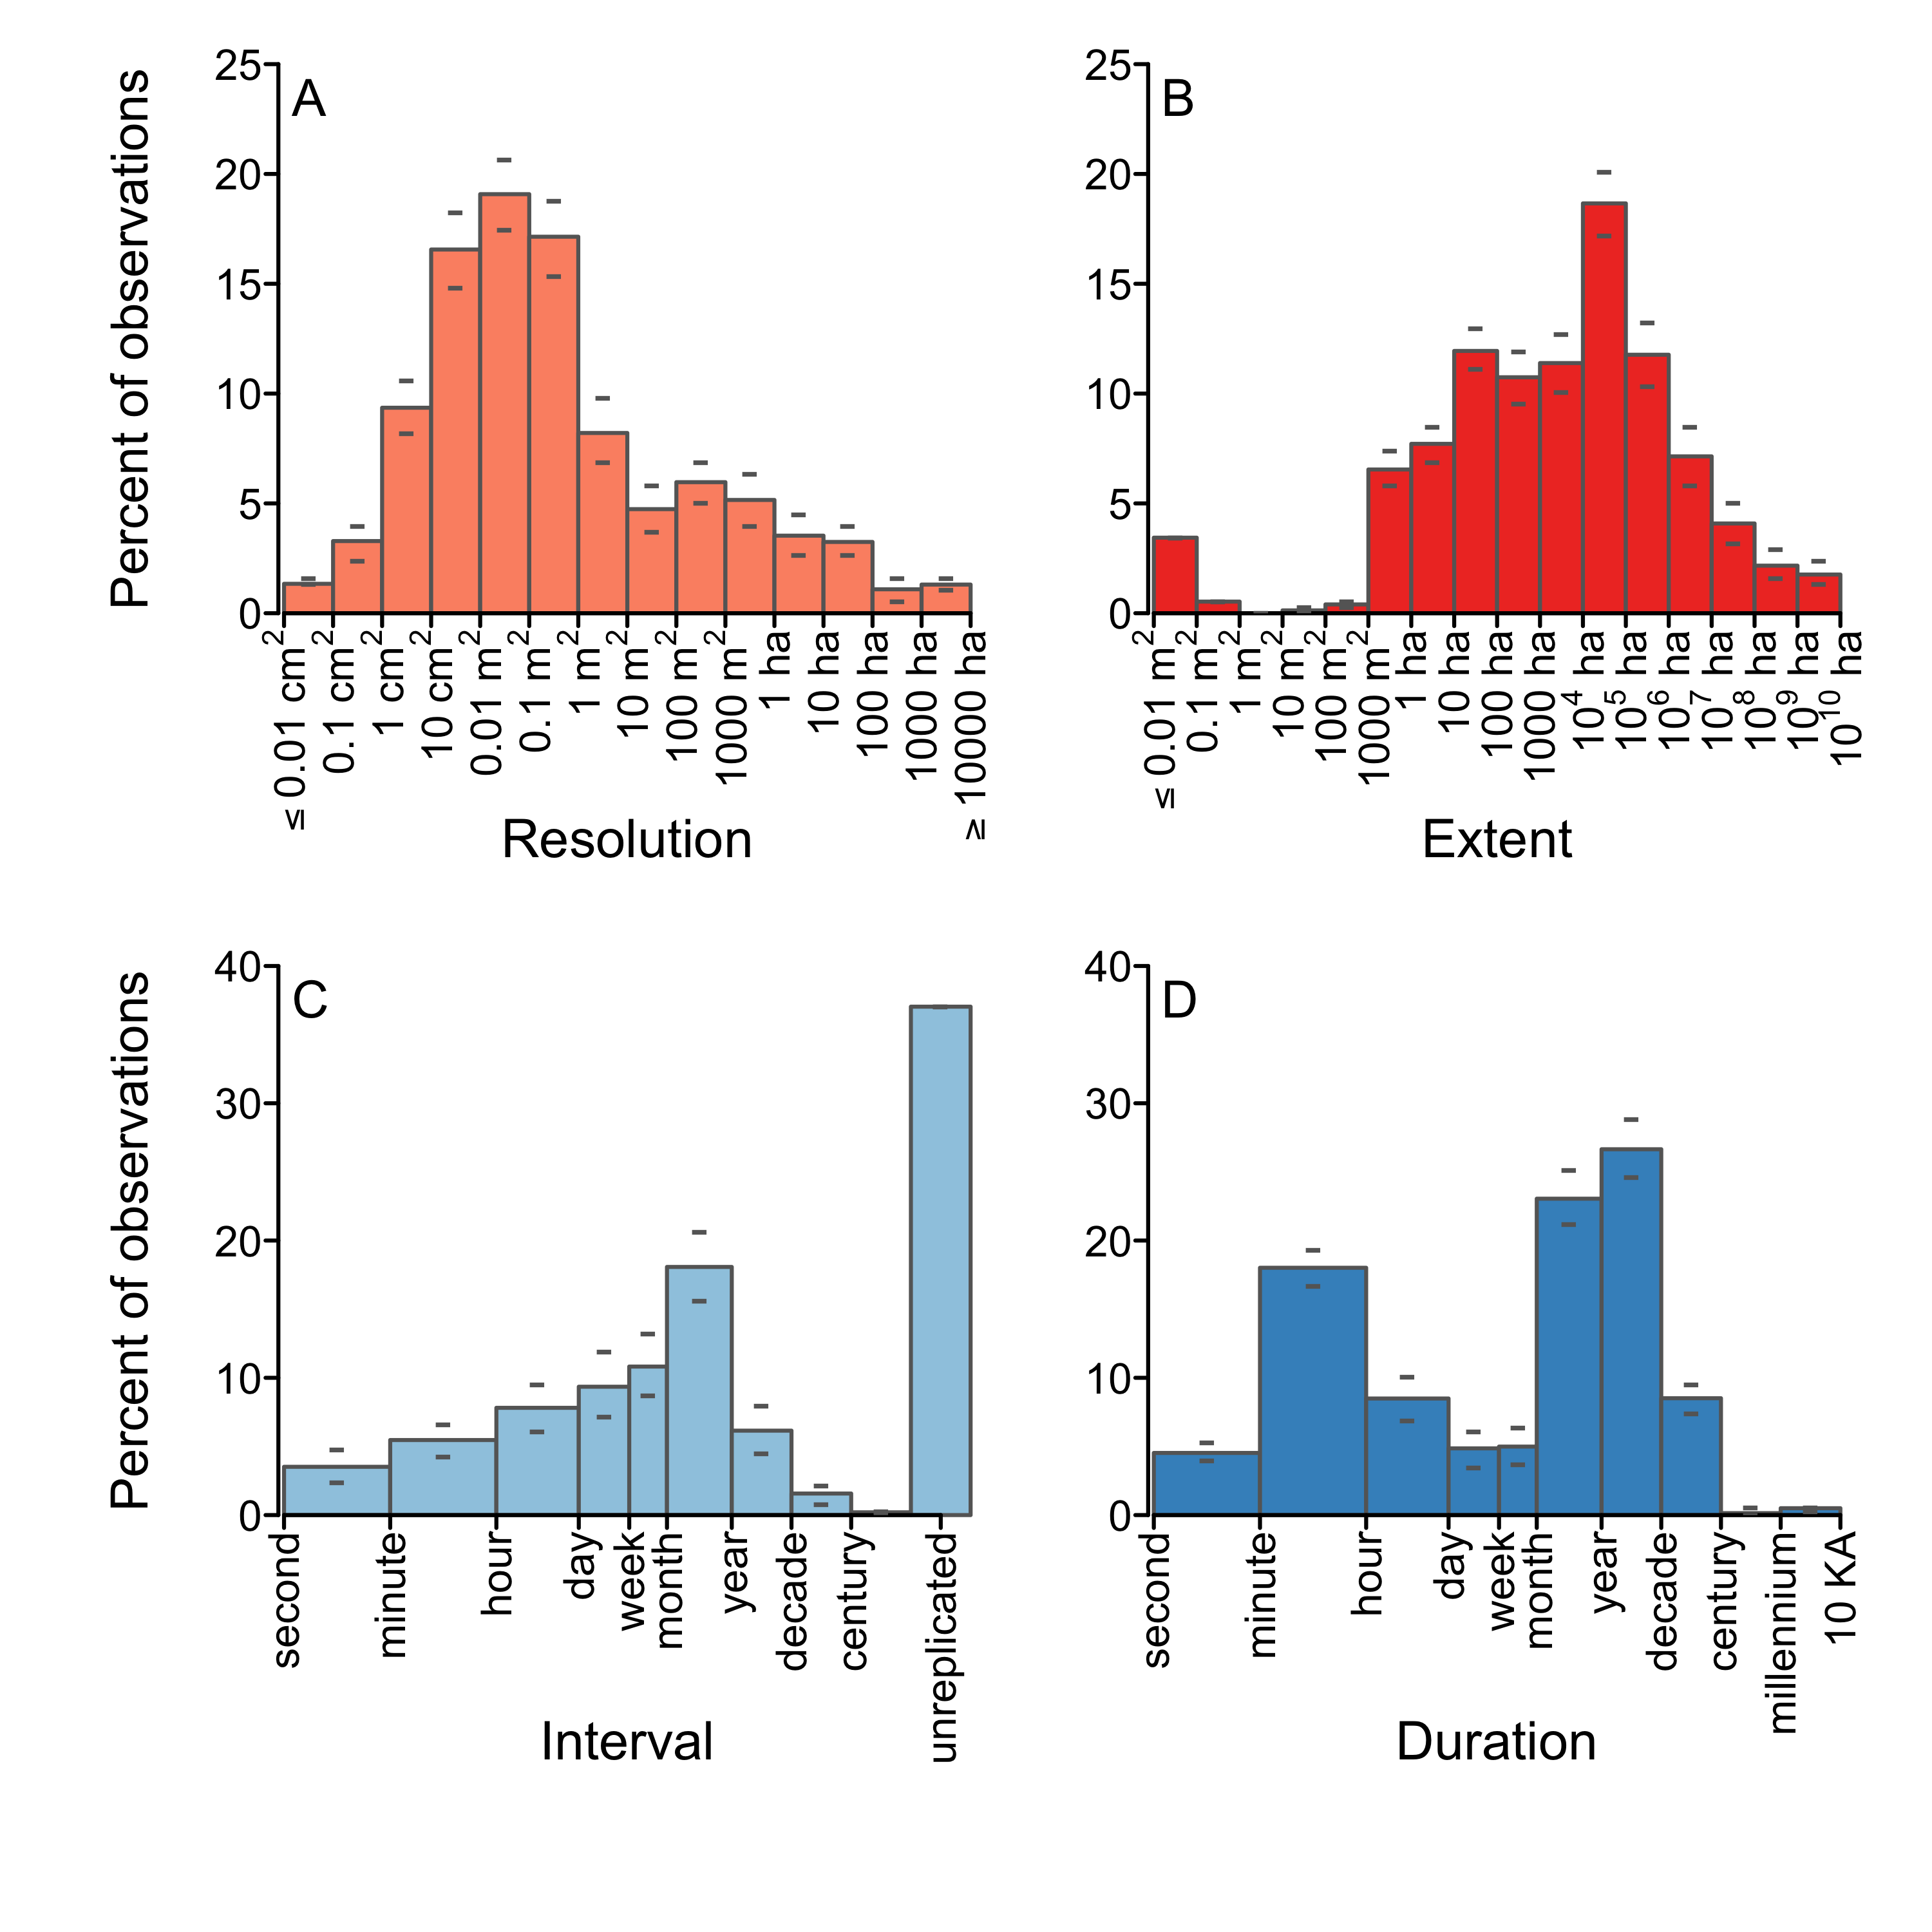
\includegraphics[width=1\textwidth]{../vignettes/figures/fig1.png}
\vspace{-0.15 cm}
\caption{Histograms of the resolution (A), extent (B), interval (C), and duration (D) of observations collected from the surveyed ecological studies. Bars represent the average percentages for each bin realized after 1000 perturbed resamples, while grey bars indicate the 95\% confidence interval. Bar widths in C-D indicate differences in scale between x-axis labels. The grey vertical line in D indicates that the majority ($>$95\%) of observations of $\leq$1 day duration were temporally unreplicated.}
\label{afoto1}
\end{figure}


\begin{figure}[!ht]
%\begin{wrapfigure}{c}{1\textwidth}
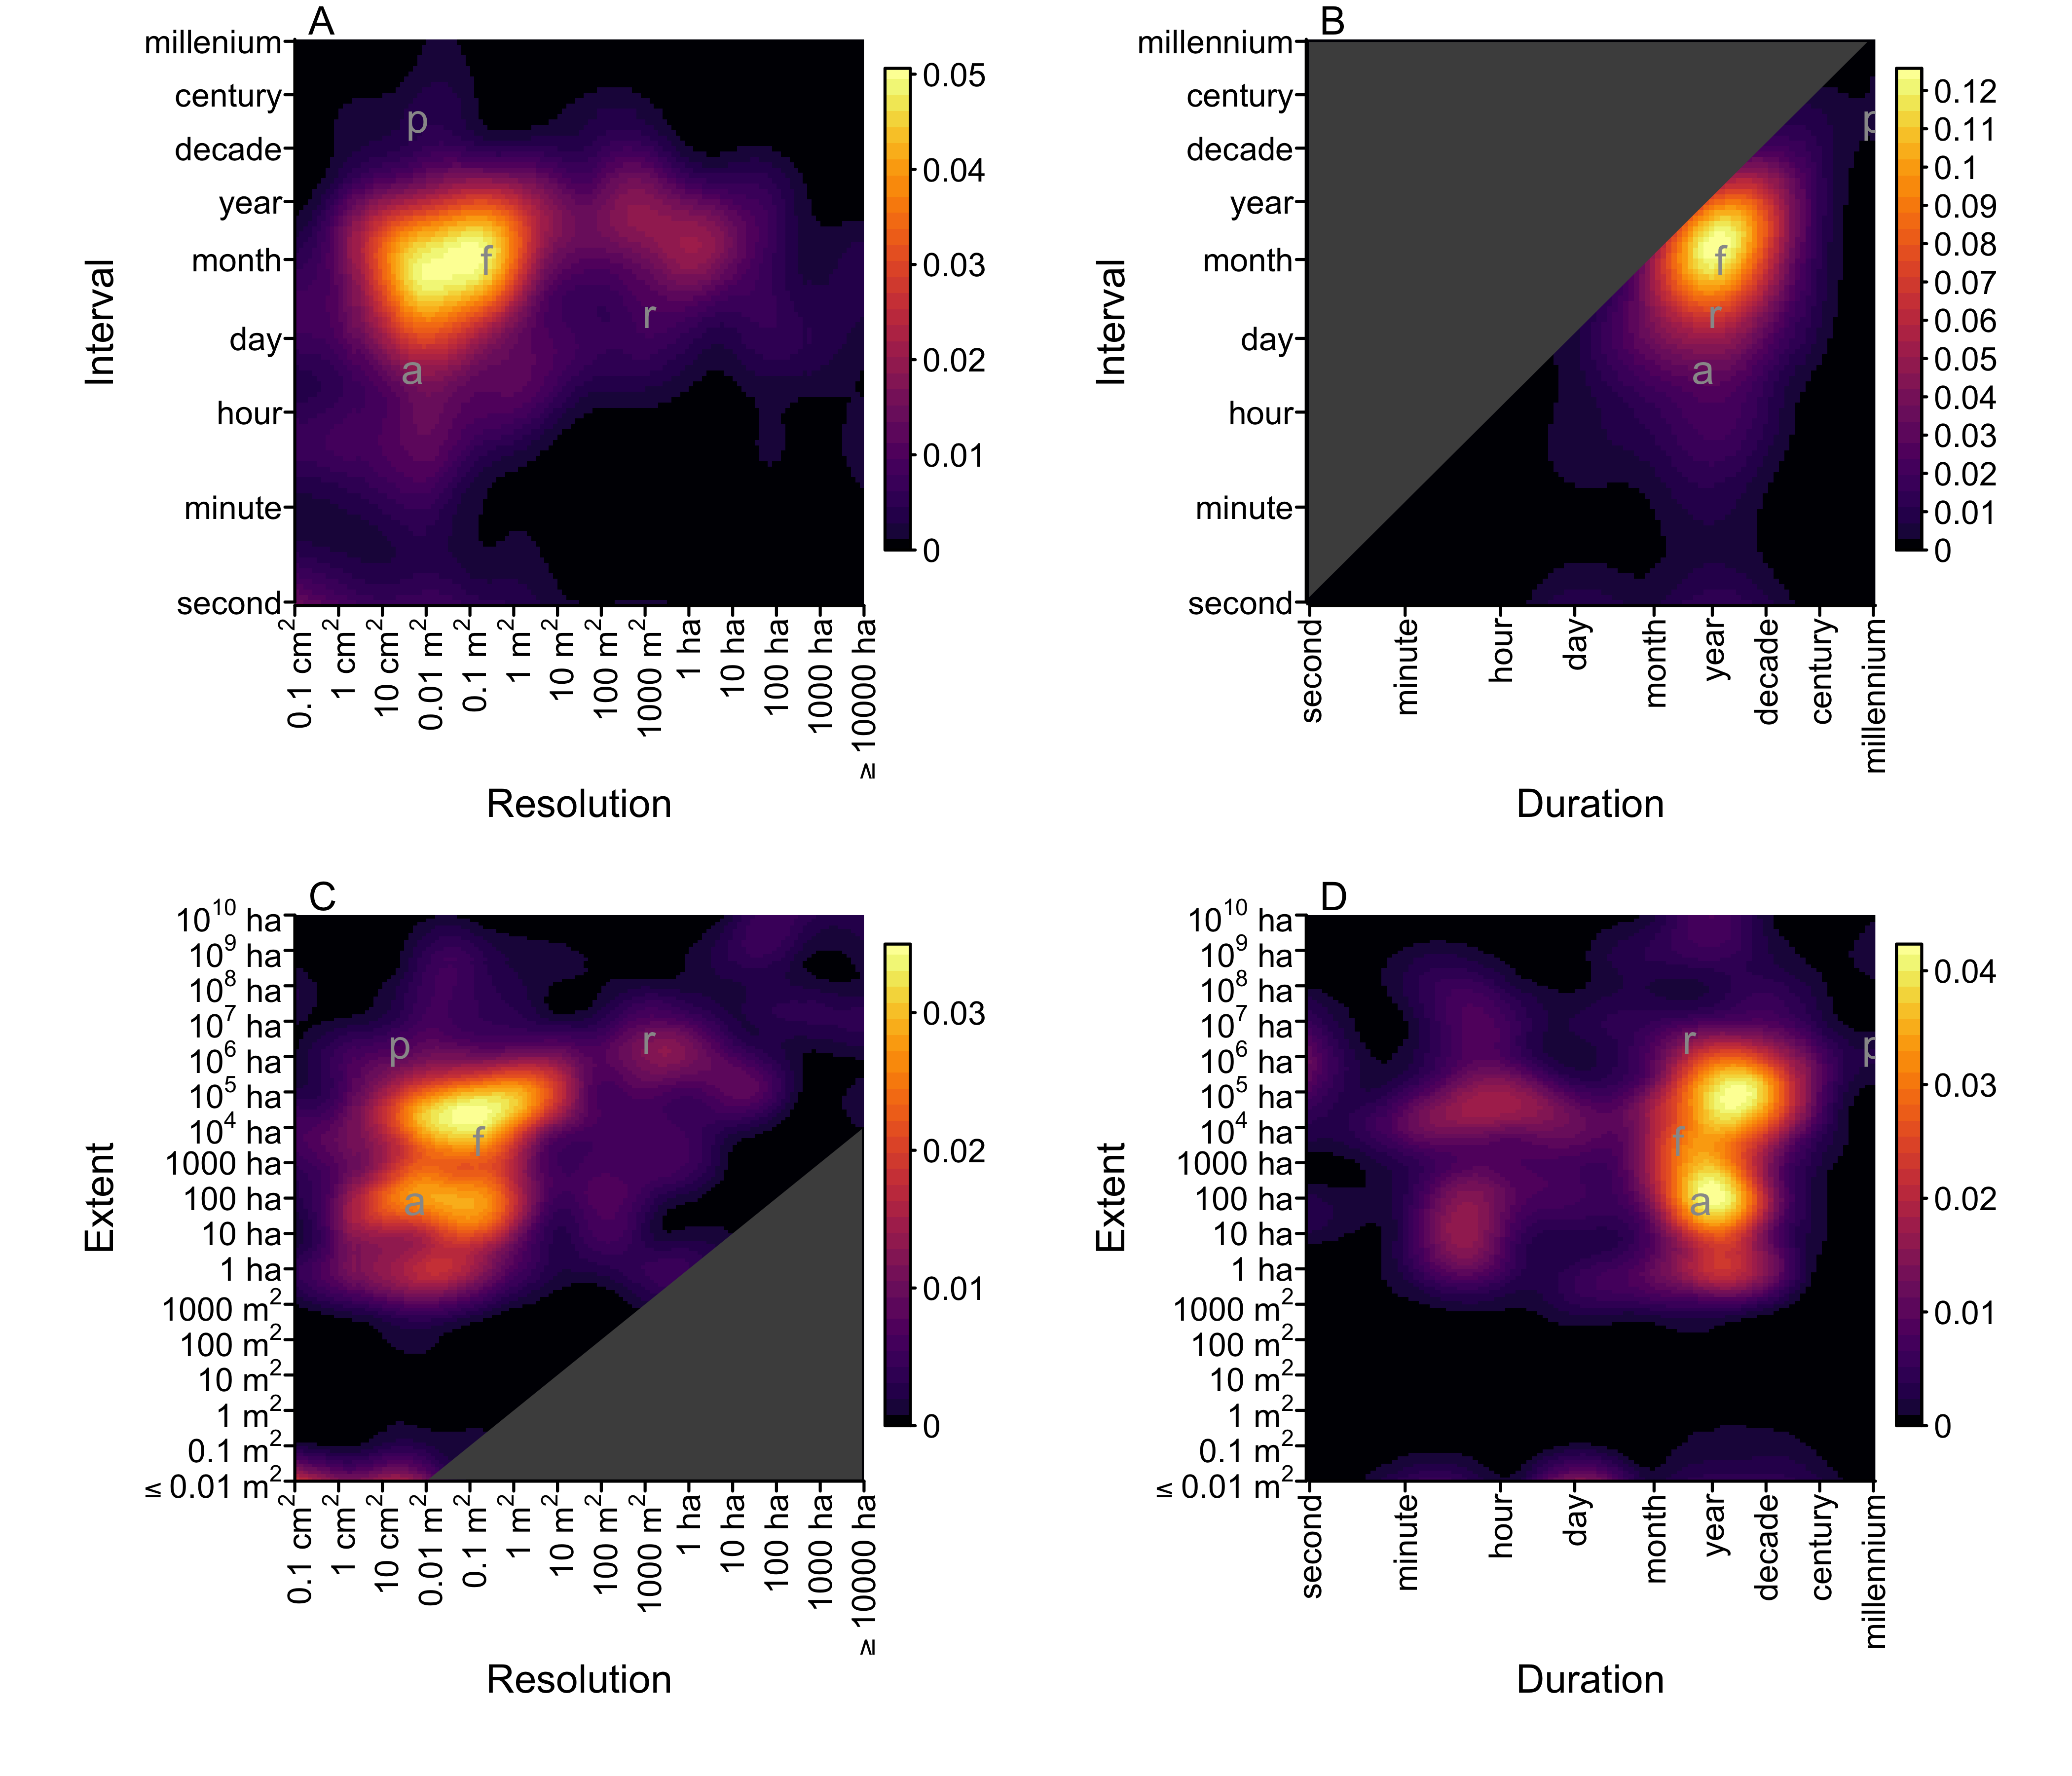
\includegraphics[width=1\textwidth]{../vignettes/figures/fig2.png}
\vspace{-0.15 cm}
\caption{Kernel density estimates of observational densities within the domains defined by A) interval and resolution (of temporally replicated observations only), B) duration and extent, C) resolution and extent, and D) interval and duration (of temporally replicated observations). Density estimates were applied to the log-transformed values of each observational dimension, and density estimates are rescaled to represent percentages. Letters in the plots denote the median values of different observational methods (f=field observations; a = automated sensing; r = remote sensing; p = paleo-observations). The grey shaded areas represent physically impossible domains (intervals greater than duration and resolutions greater than extent).}
\label{afoto1}
\end{figure}

\begin{figure}[ht]
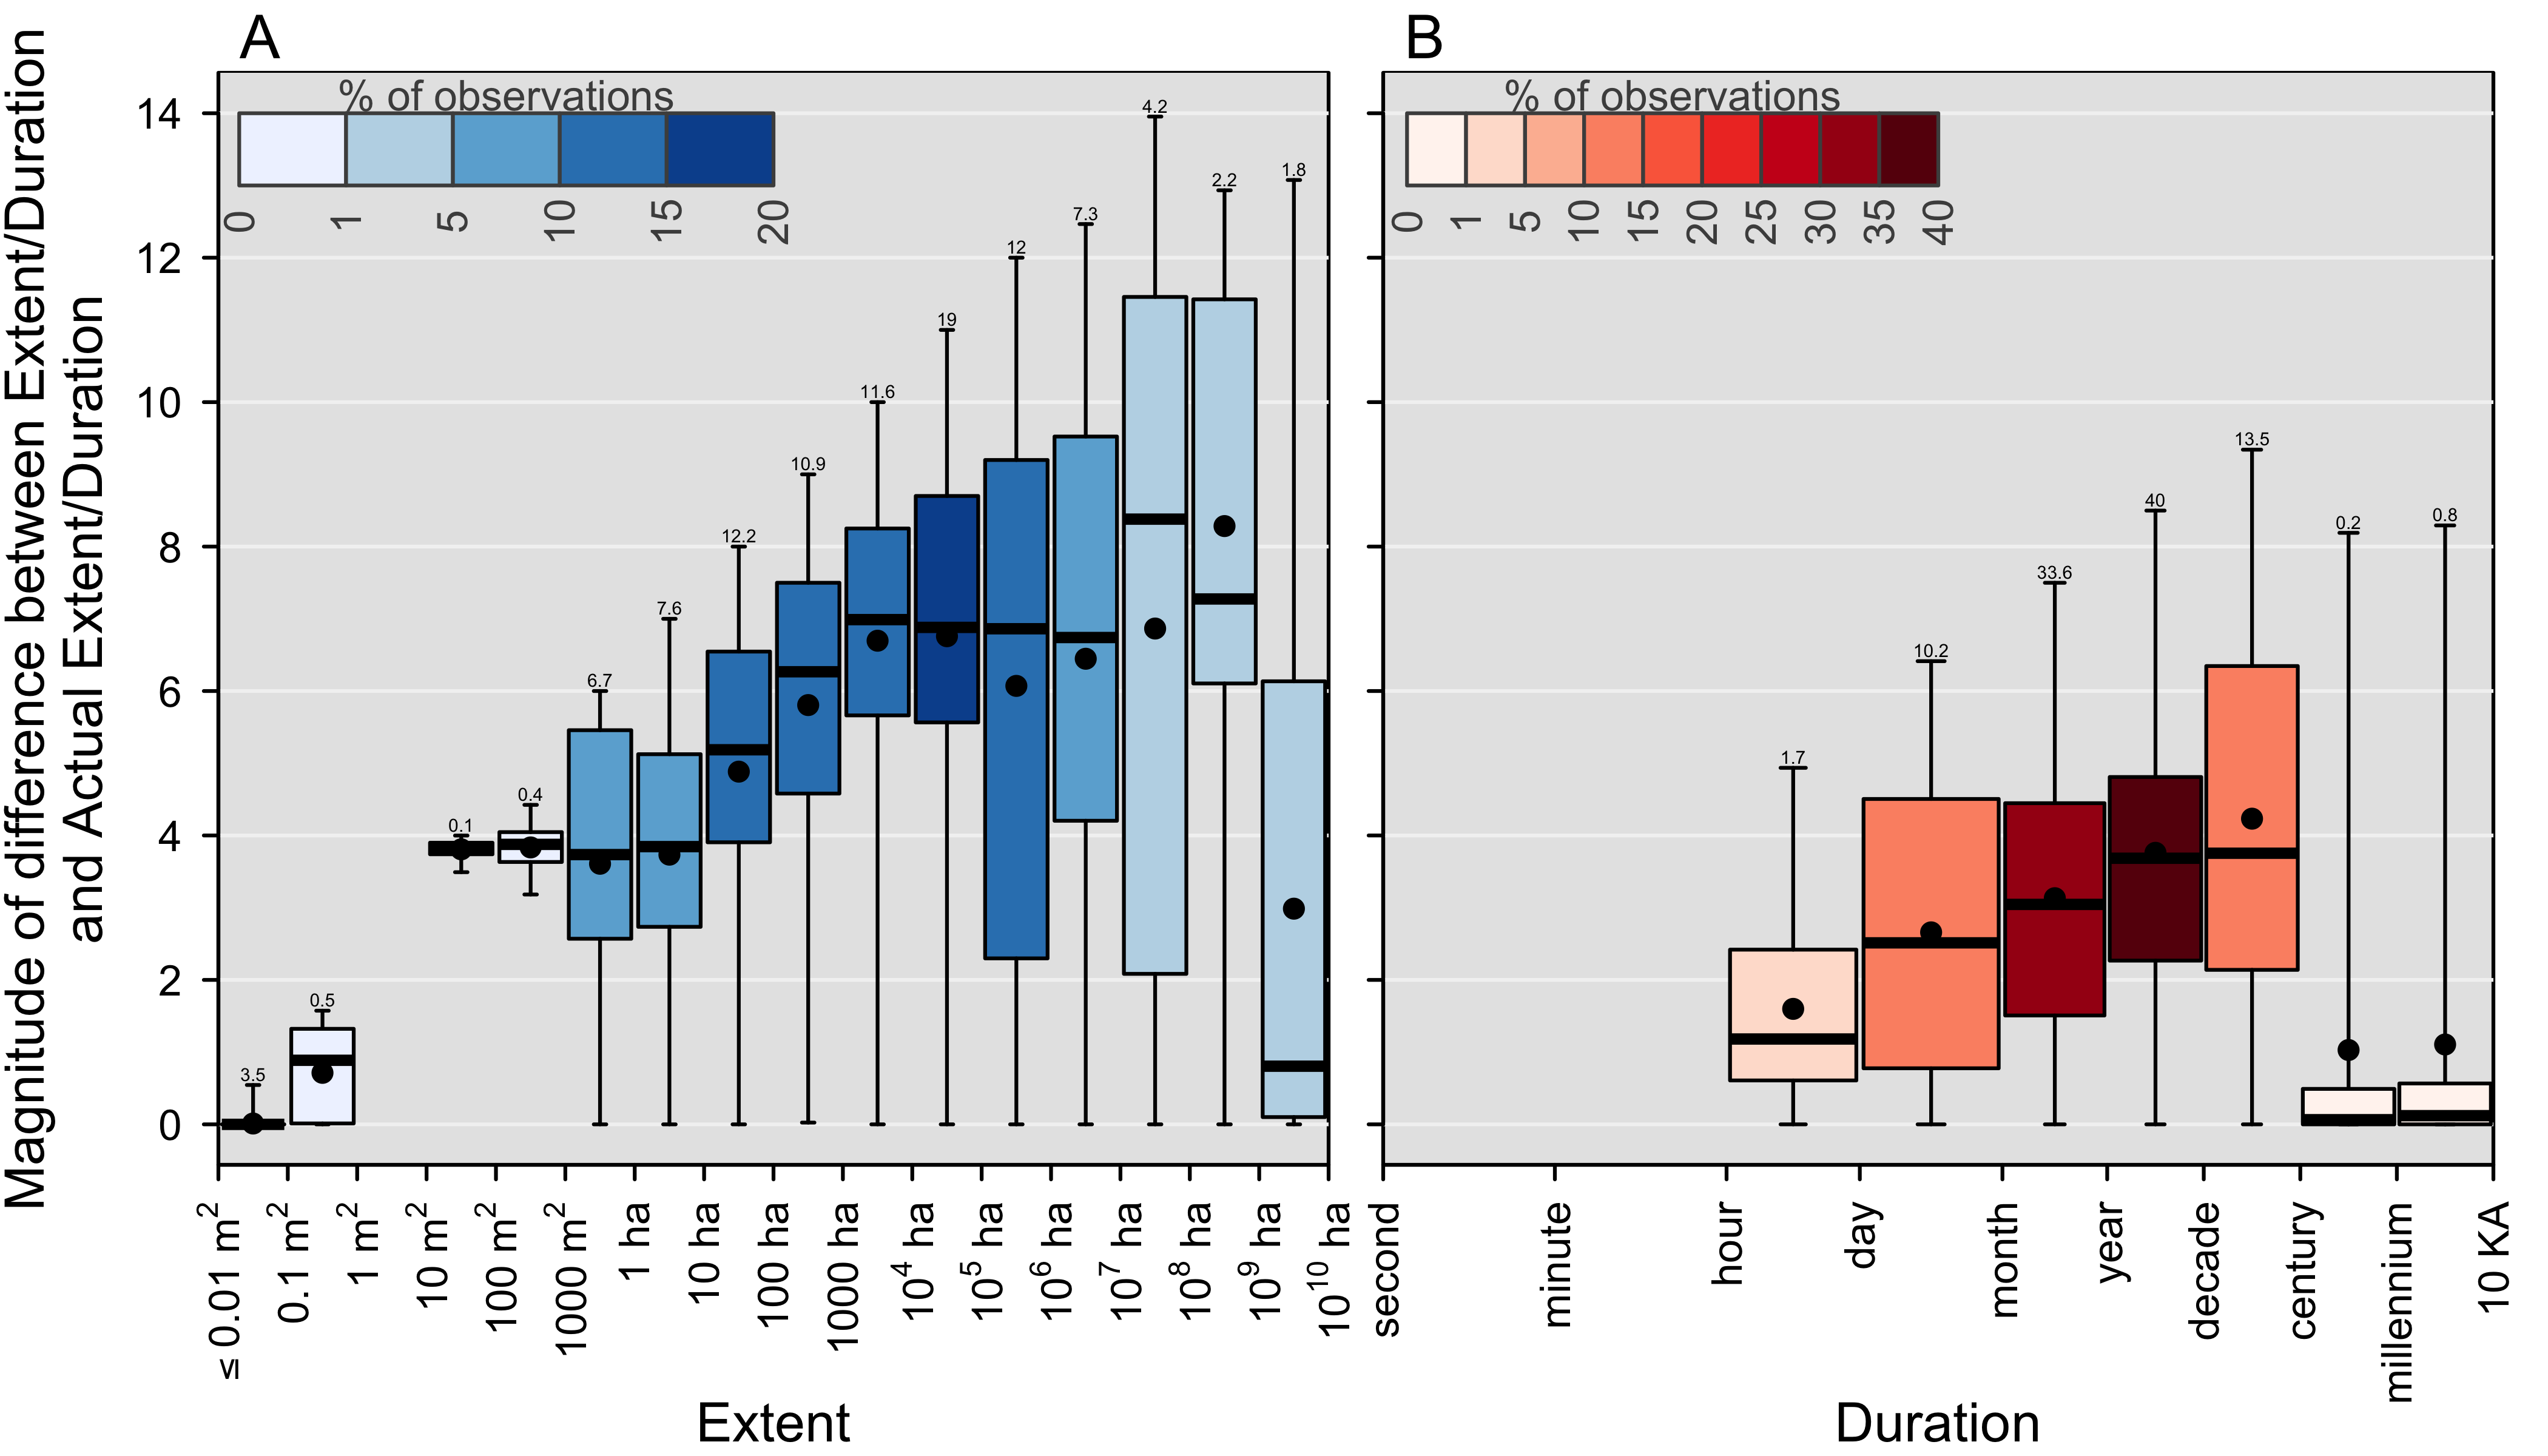
\includegraphics[width=1\textwidth]{../vignettes/figures/fig3.png}
\vspace{-0.2 cm}
\caption{The difference between extent and \emph{actual} extent (the summed area of spatial replicates) (A) and duration and \emph{actual} duration (the summed sampling duration across temporal replicates) (B). Difference values are expressed in terms of how many orders of magnitude larger (or longer) extent (duration) is than actual extent (actual duration), and are summarized (as box plots, with circle in box representing the mean and line the median) in bins representing increasing scales of actual extent/duration.  The percentages of observations falling within each bin are indicated by the color of the inter-quartile and the numeric value above the upper whisker. The grey vertical line in D indicates that the majority ($>$95\%) of observations of $\leq$1 day duration were temporally unreplicated.}
\label{afoto1}
\end{figure}


\end{document}




















